\documentclass[a4paper]{jsarticle}
\usepackage[dvipdfmx]{graphicx}
\usepackage{wrapfig}
\usepackage{amsmath}
\usepackage{subfigure}
\usepackage{listings}
\usepackage{ascmac}
\usepackage{txfonts}

\setlength{\topmargin}{3.6truemm}
\setlength{\oddsidemargin}{3.6truemm}
\setlength{\evensidemargin}{3.6truemm}
\setlength{\headheight}{0truemm}
\setlength{\headsep}{0truemm}
\setlength{\textheight}{25.5truecm}
\setlength{\textwidth}{15.5truecm}


%
\setlength{\parindent}{1zw}
%
\usepackage{graphicx}
\usepackage{wrapfig}
\makeatletter
\def \fgcaption{\def \@captype{figure} \caption}
\def \tbcaption{\def \@captype{table} \caption}
\makeatother
%\def \figurename{Fig.}
%\def \tablename{Table}
\def\linesparpage#1{
\baselineskip=\textheight
\divide\baselineskip by #1
}
%
\hyphenpenalty=10000\relax
\exhyphenpenalty=10000\relax
\sloppy
%
\def\topfraction{.95}
\def\bottomfraction{.95}
\def\textfraction{.05}
\def\floatpagefraction{.8}
\def\dbltopfraction{.95}
\def\dbltextfraction{.05}
\def\dblfloatpagefraction{.8}

%
\pagestyle{empty}
%
\begin{document}

\fontsize{11pt}{20pt}\selectfont

\begin{center}
{\huge 情報可視化論 最終課題}
\end{center}
\begin{flushright}
{\Large 2017 / 06 / 16(Fri)}
\end{flushright}
\begin{flushright}
{\Large 171X012X \hspace{16pt} 早田 一}
\end{flushright}

\par
今回は,No.15で紹介されたIsovalueの値をスライドバーで変更できるロブスターデータ(http://naohisas.github.io/KVS.js/Example/MarchingCubes/)に,以下の2つの機能を加えた.
\begin{itemize}
\item Isovalueのバーに加え,Colorのバーを設けた. \\
これにより,Isovalueの値からロブスターの色を与えていたものを,Isovalueで等値面値の身の変更を行い,色の変更を独自にできるようにした.
\item ロブスターデータに加え,ハイドロゲンデータ(水素分子データ)を可視化できるようにした.\\
また,2つのデータを選択ボックスで選択できるようにした.
\end{itemize}
\par
また,今回は初期状態を空のボックスに設定し,2つのデータ選択を元にボックスのサイズを調整するようにした.
各状態を以下の図に示す.
\vspace{25pt}
\begin{figure}[htbp]
\begin{center}
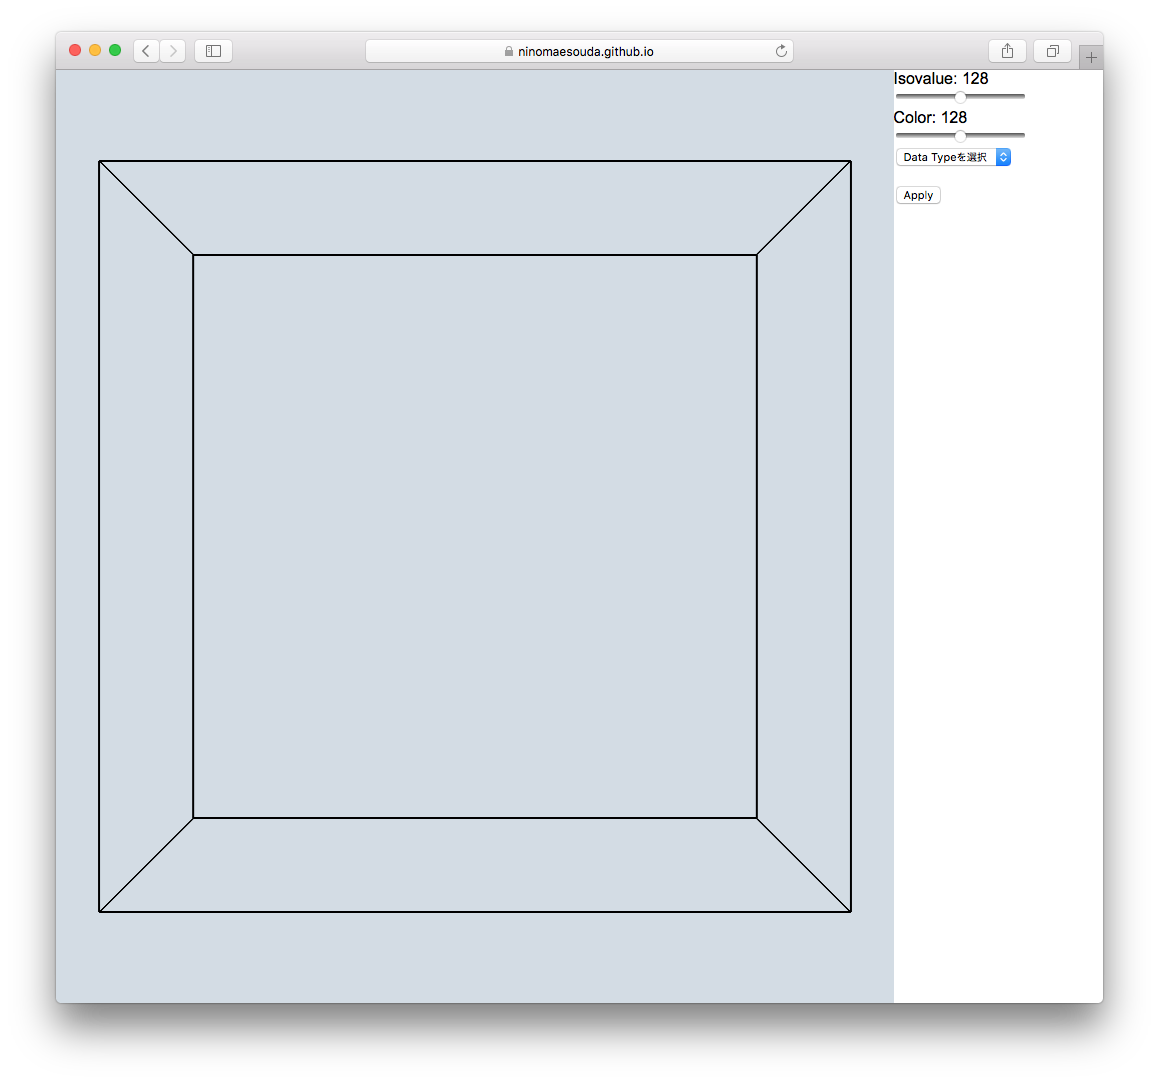
\includegraphics[scale = 0.18]{vis_first.png}
\\ 初期状態
\end{center}
\end{figure}

\begin{figure}[htbp]
\begin{minipage}{0.5\hsize}
\begin{center}
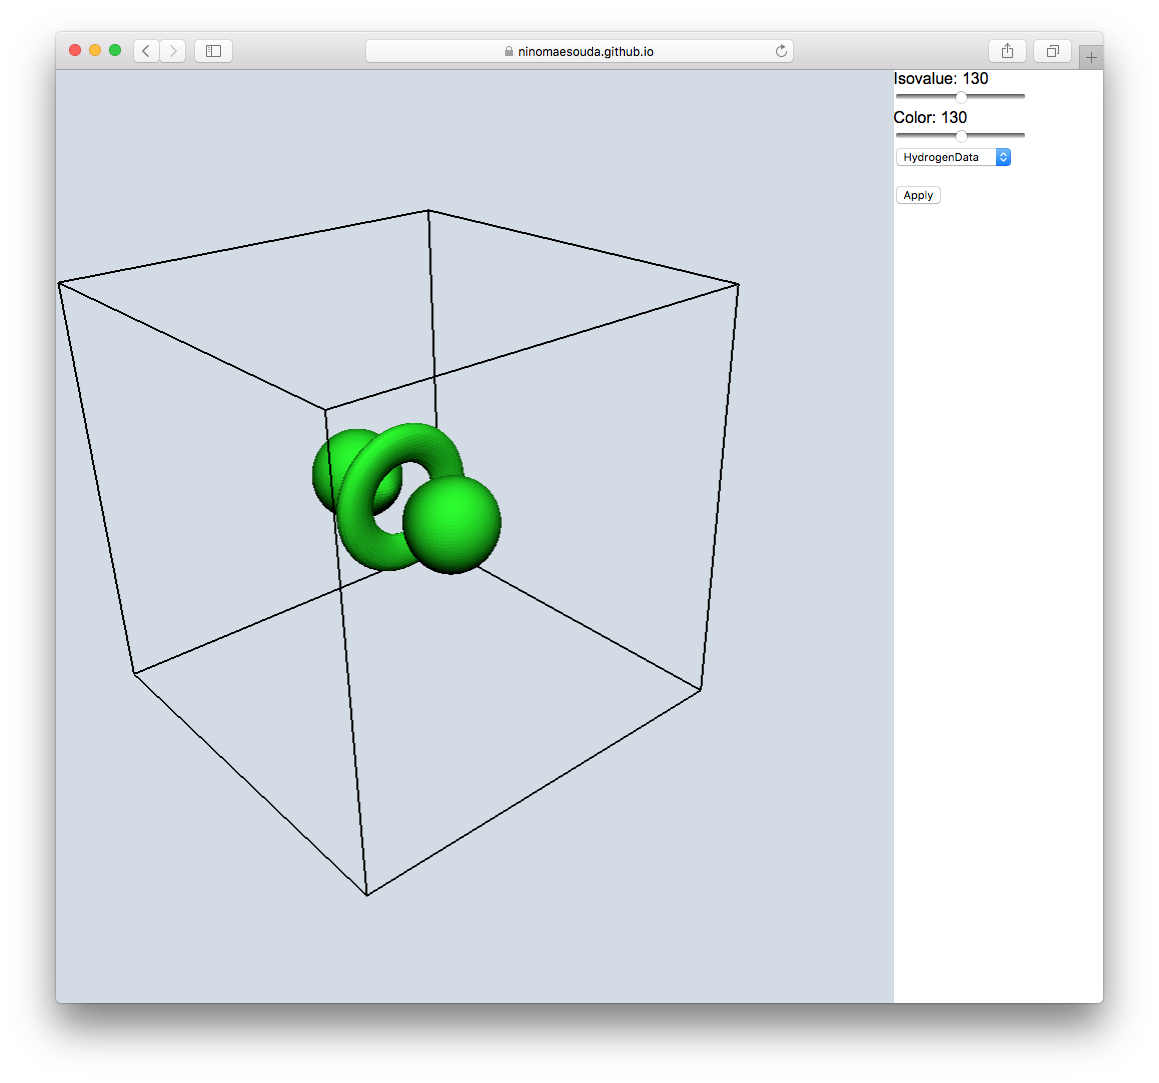
\includegraphics[scale = 0.18]{vis_hyd1.png}
\\ Hydrogen (Isovalue : 130, Color : 130)
\end{center}
\end{minipage}
\begin{minipage}{0.5\hsize}
\begin{center}
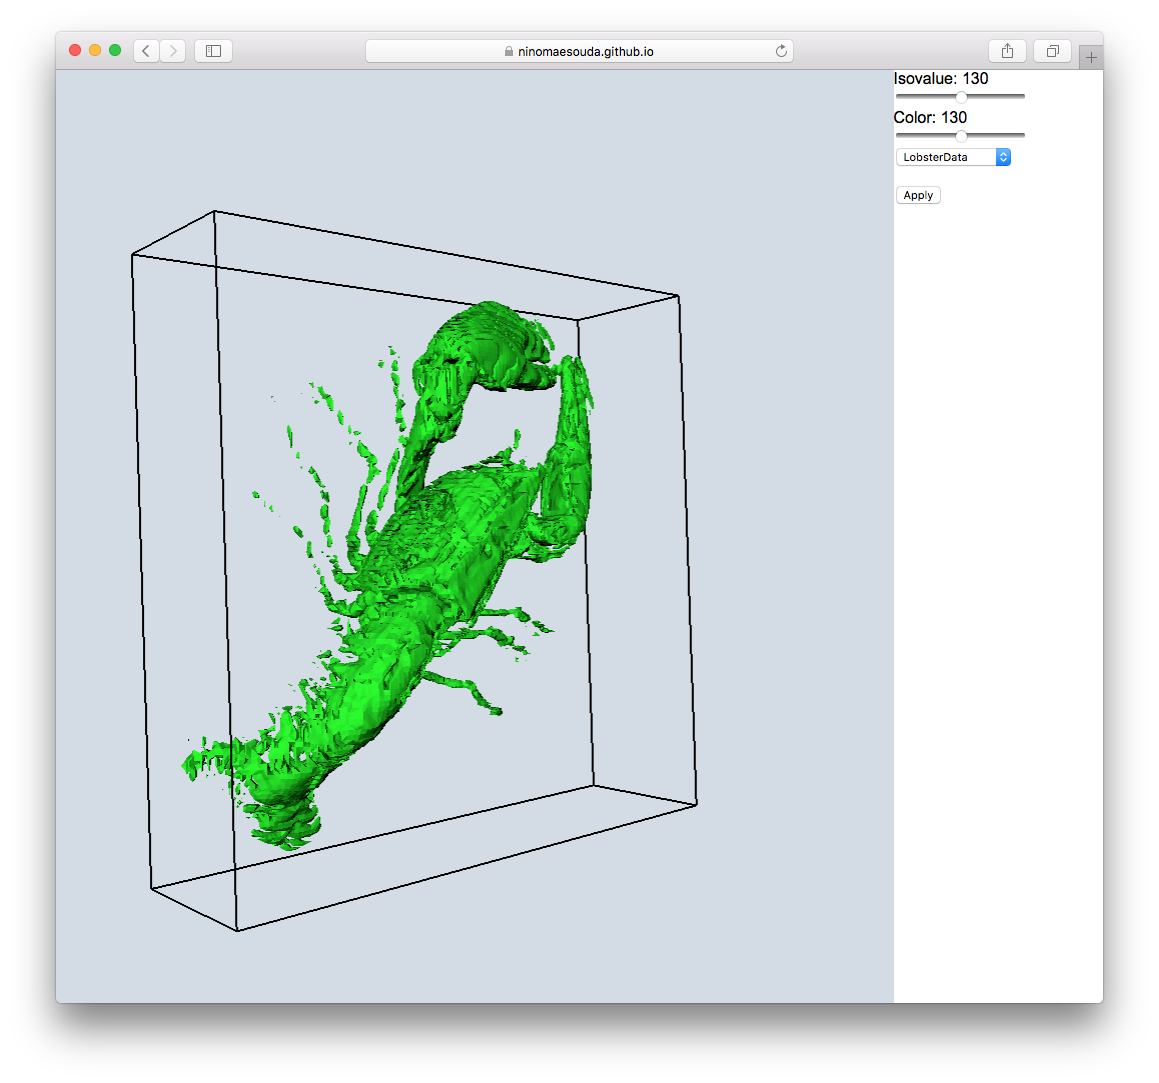
\includegraphics[scale = 0.18]{vis_lob1.png}
\\ Lobster (Isovalue : 130, Color : 130)
\end{center}
\end{minipage}
\end{figure}

\begin{figure}[htbp]
\begin{minipage}{0.5\hsize}
\begin{center}
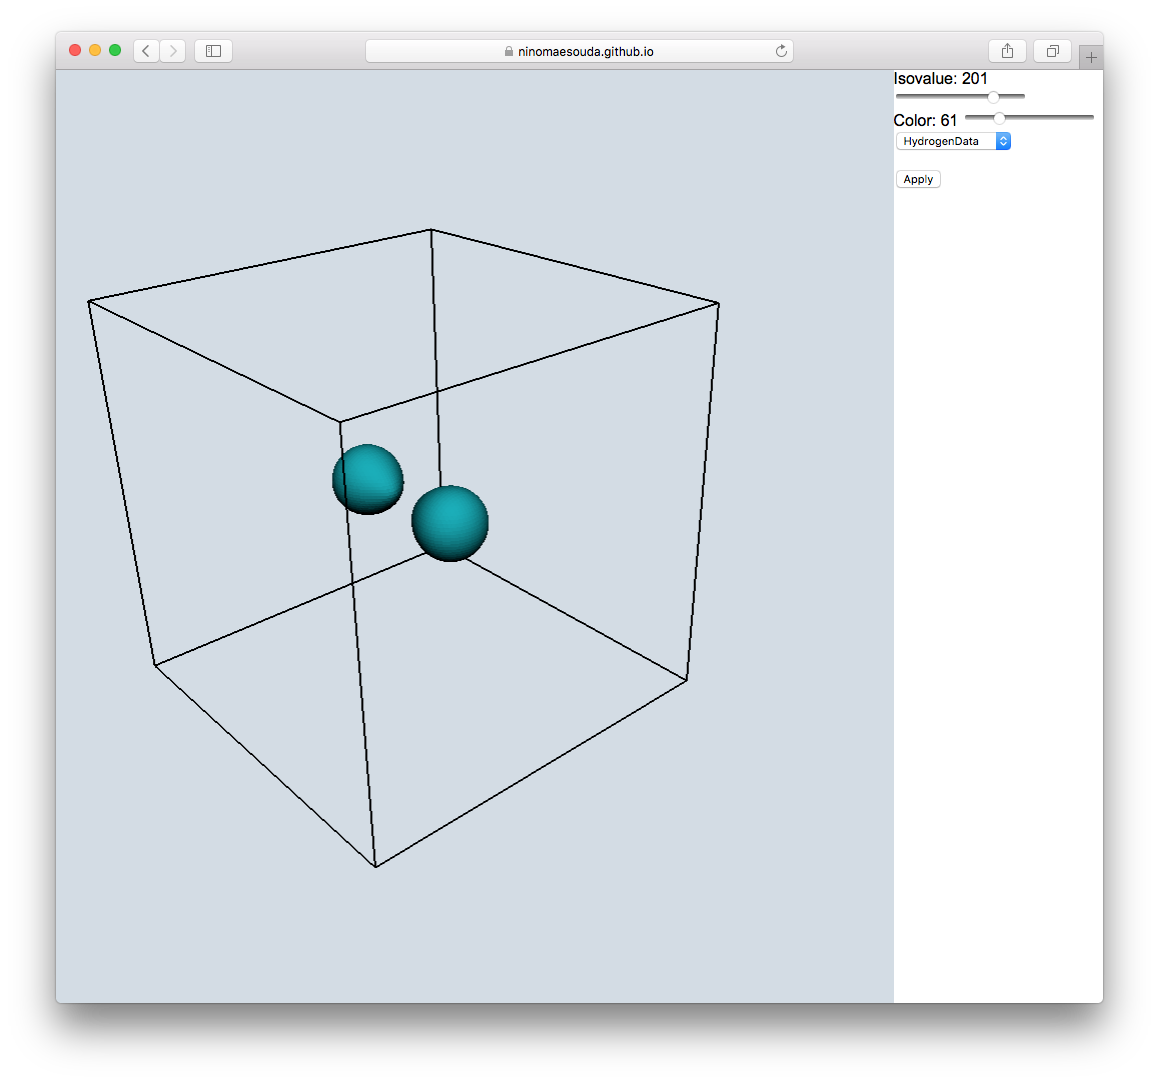
\includegraphics[scale = 0.18]{vis_hyd2.png}
\\ Hydrogen (Isovalue : 201, Color : 61)
\end{center}
\end{minipage}
\begin{minipage}{0.5\hsize}
\begin{center}
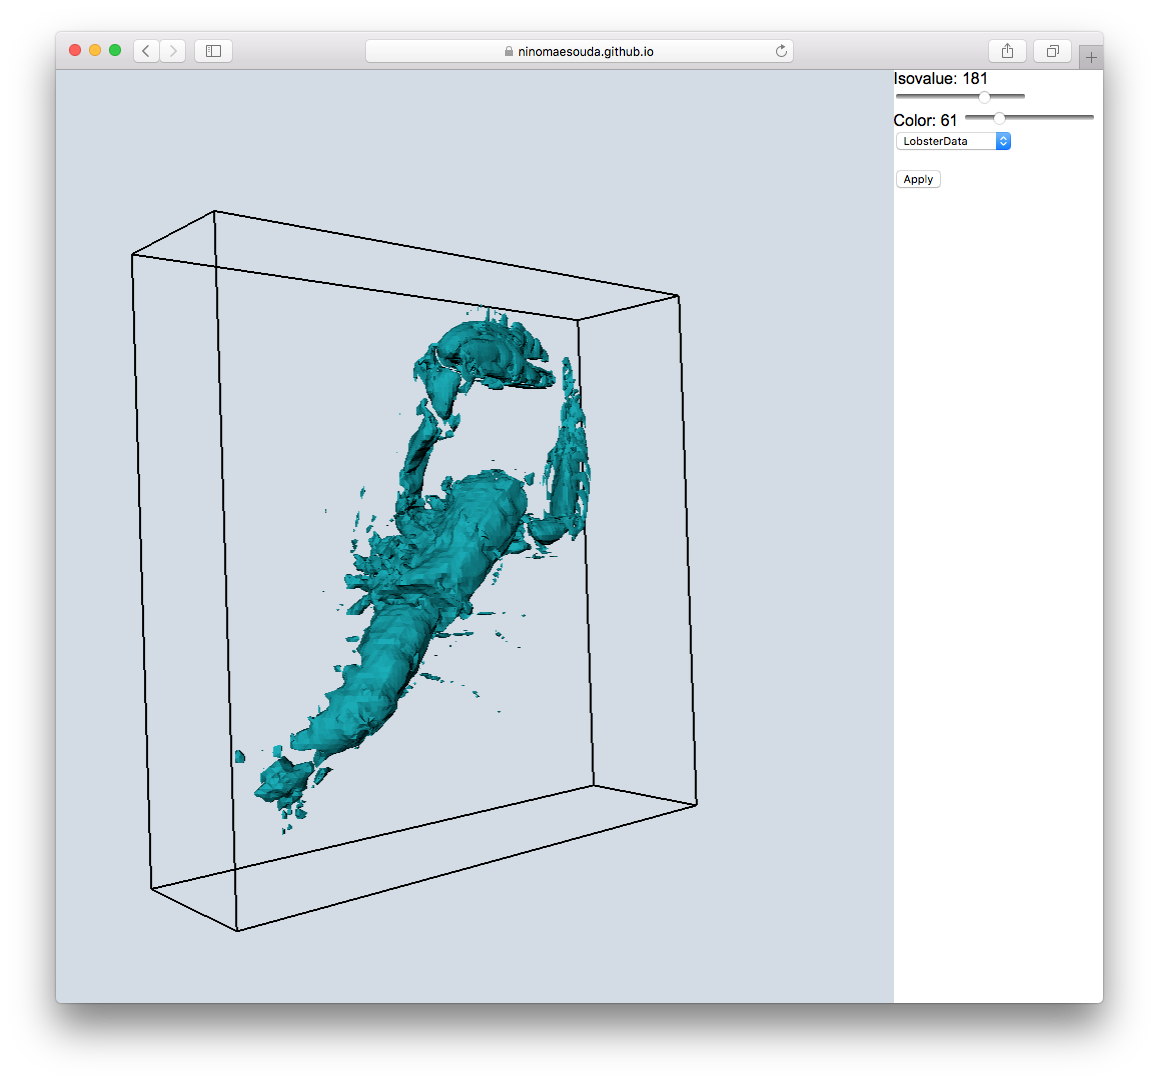
\includegraphics[scale = 0.18]{vis_lob2.png}
\\ Lobster (Isovalue : 181, Color : 61)
\end{center}
\end{minipage}
\end{figure}

\begin{figure}[htbp]
\begin{minipage}{0.5\hsize}
\begin{center}
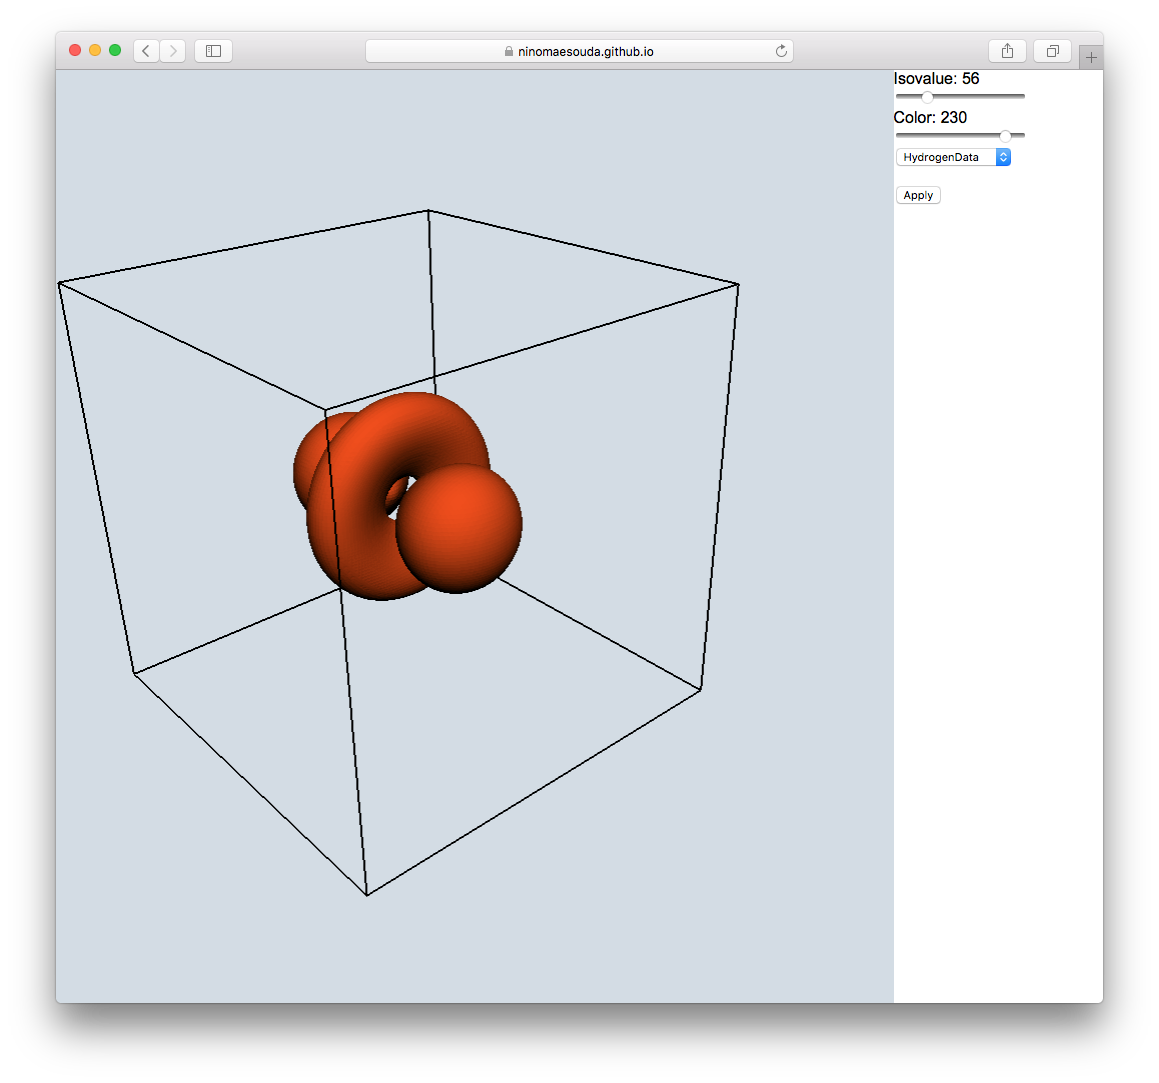
\includegraphics[scale = 0.18]{vis_hyd3.png}
\\ Hydrogen (Isovalue : 56, Color : 230)
\end{center}
\end{minipage}
\begin{minipage}{0.5\hsize}
\begin{center}
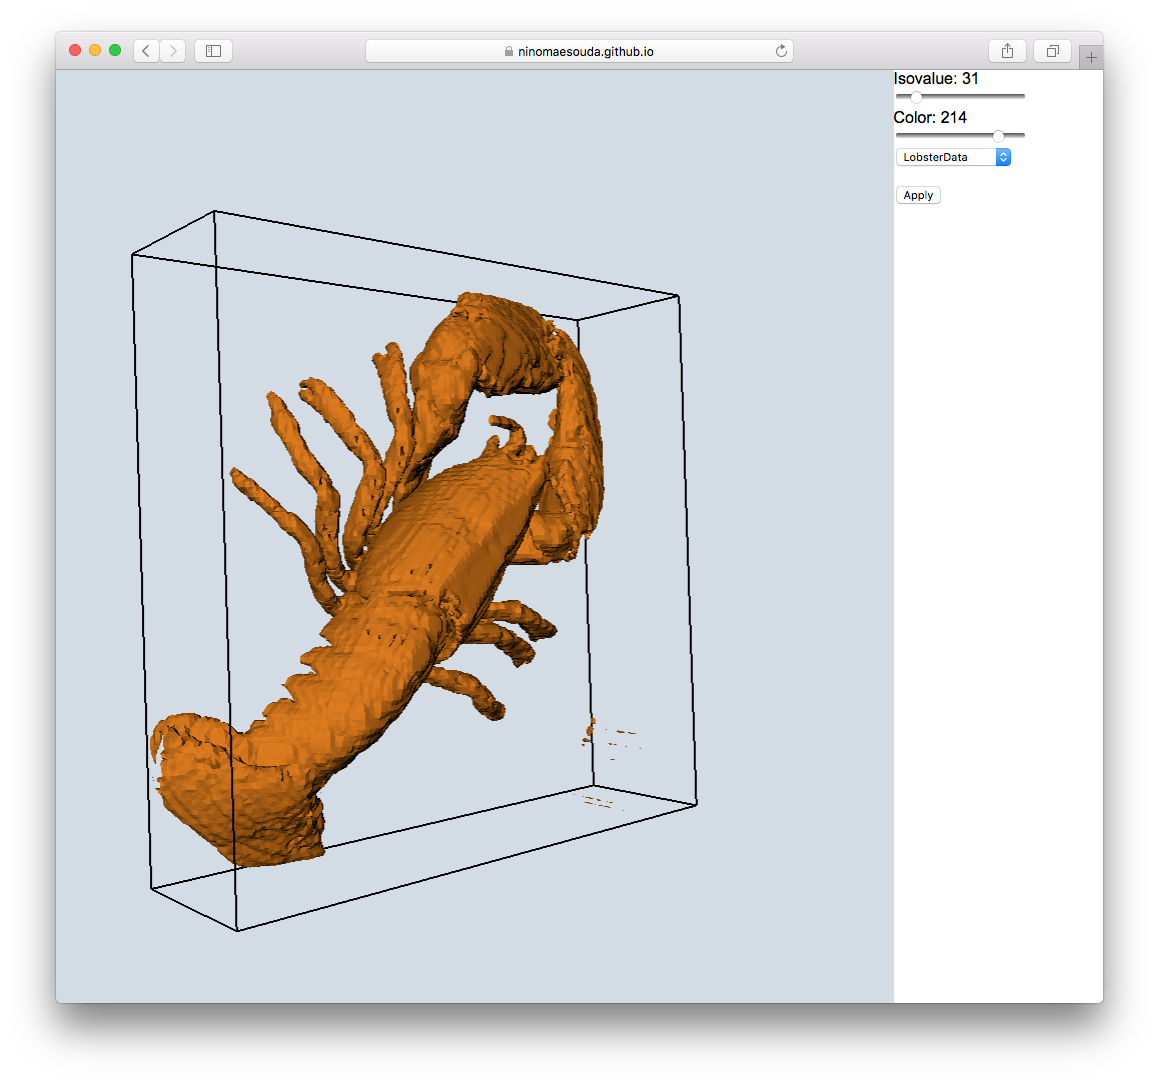
\includegraphics[scale = 0.18]{vis_lob3.png}
\\ Lobster (Isovalue : 31, Color : 214)
\end{center}
\end{minipage}
\end{figure}

\end{document}